% BACSE324 Review 2 — Data Glove Gesture Recognition System
% Compile: pdflatex report.tex (twice, for TOC/refs) 
\documentclass[11pt,a4paper]{article}

\usepackage[margin=2cm]{geometry}
\usepackage[table]{xcolor}
\usepackage{booktabs}
\usepackage{tabularx}
\usepackage{array}
\usepackage{enumitem}
\usepackage{titlesec}
\usepackage{fancyhdr}
\usepackage{graphicx}
\usepackage{float}
\usepackage{amsmath}
\usepackage[colorlinks=true,linkcolor=black,urlcolor=blue]{hyperref}
\usepackage{parskip}

% ---- colours (match the docx template: dark header, warm paper) ----
\definecolor{headbg}{HTML}{1C1B19}
\definecolor{headfg}{HTML}{FFFFFF}
\definecolor{rowalt}{HTML}{F4F2EC}
\definecolor{kicker}{HTML}{6B675F}

% ---- heading style ----
\titleformat{\section}{\Large\bfseries}{\thesection}{0.6em}{}
\titleformat{\subsection}{\large\bfseries}{\thesubsection}{0.6em}{}
\titlespacing{\section}{0pt}{14pt}{6pt}
\titlespacing{\subsection}{0pt}{10pt}{4pt}

% ---- header table helper: dark header row ----
\newcommand{\hdrow}[1]{\rowcolor{headbg}\color{headfg}\bfseries #1}
\renewcommand{\arraystretch}{1.25}

% ---- footer ----
\pagestyle{fancy}
\fancyhf{}
\renewcommand{\headrulewidth}{0pt}
\fancyfoot[L]{\footnotesize\color{kicker}BACSE324 · Review 2 · Data Glove}
\fancyfoot[R]{\footnotesize\color{kicker}\thepage}

\title{\vspace{-1.2cm}\textbf{Design Models: CDFG, FSM and Task Schedule}\\[4pt]
\large Gesture-Controlled Smart Glove for Human–Computer Interaction\\[2pt]
\normalsize BACSE324 · Embedded Systems Architecture · Fall 2026 · Review 2}
\date{}

\begin{document}
\maketitle
\vspace{-1.0cm}

% ===================== COVER TABLE =====================
\begin{tabularx}{\textwidth}{@{}>{\bfseries}p{4.2cm}X@{}}
\hdrow{Field & Value} \\[1pt]
Project title & Gesture-Controlled Smart Glove for Human–Computer Interaction \\
Scope tier & Tier 2 — full embedded system \\
Submission date & September 2026 \\
Repository & \texttt{github.com/dayaj1222/data-glove} \\
\end{tabularx}

\vspace{8pt}
\begin{tabularx}{\textwidth}{@{}p{4.2cm}p{2.6cm}X@{}}
\hdrow{Member & Reg.\ no. & Module owned / sections} \\[1pt]
Dayakrishn Joshi & 25BCE2951 & ESP-32 firmware, MPU-9250 I²C + flex ADC acquisition — §1, §2, §4 \\
Syed Mohammad Ayaan & 25BCE2311 & ESP-32 wireless link, PC recognition pipeline — §3, §5, §6, §7 \\
\end{tabularx}

\vspace{6pt}
{\footnotesize\color{kicker}Diagrams are our own (Excalidraw and TikZ). Every timing figure
is labelled measured, datasheet, or estimated.}

% ===================== 1 SYSTEM RECAP =====================
\section{System recap}

The Smart Glove is a wearable input device that converts hand pose (two flex
sensors) and hand motion (an MPU-9250 9-axis IMU) into standard keyboard and
mouse events on a PC, for a single operator who wants hands-free control. The
ESP-32 firmware samples both flex ADC channels and the IMU over
I\textsuperscript{2}C at a fixed rate and frames them into a fixed-width binary
record: five 16-bit flex counts followed by nine 32-bit floats
(accelerometer $x,y,z$, gyroscope $x,y,z$, magnetometer $x,y,z$) --- a 58-byte
datagram, parsed on the host by
\texttt{glove/protocol/simple.py::SimpleBinaryProtocol.parse} using the
\texttt{<5H9f} struct format. Frames arrive over UDP (default port 5005) through
\texttt{glove/transport/udp.py::UDPTransport.recv}, are pushed through
\texttt{glove/pipeline/main.py::Pipeline.run}, classified, and dispatched to an
action binding. On the PC a portable recognition layer classifies the gesture and
an OS-specific layer injects it as input (uinput on Linux, SendInput on Windows).
The host pipeline is transport- and recogniser-agnostic --- \texttt{Transport},
\texttt{Protocol}, \texttt{Recognizer} and \texttt{Action} are all interfaces
--- so the same code runs against the mock transport used in unit tests and the
live UDP link.

\noindent\textbf{Deviations from the approved proposal.} Two changes were made
at the design stage and are stated here so the models below are read against
what is built, not what was proposed: (i) the proposed MPU6050 was replaced by
the \textbf{MPU-9250} (9-axis, I\textsuperscript{2}C) for its on-board
magnetometer and better availability; (ii) only \textbf{two flex sensors} are
fitted rather than five --- flex sensors are the most expensive part, and two
(index + thumb) are sufficient to demonstrate distinct poses for a
proof-of-concept. The wire format already carries five flex slots, so the two
fitted sensors populate flex[0] and flex[1] and the remaining slots read zero;
no host change is needed when the other three are added.

\begin{figure}[H]
\centering
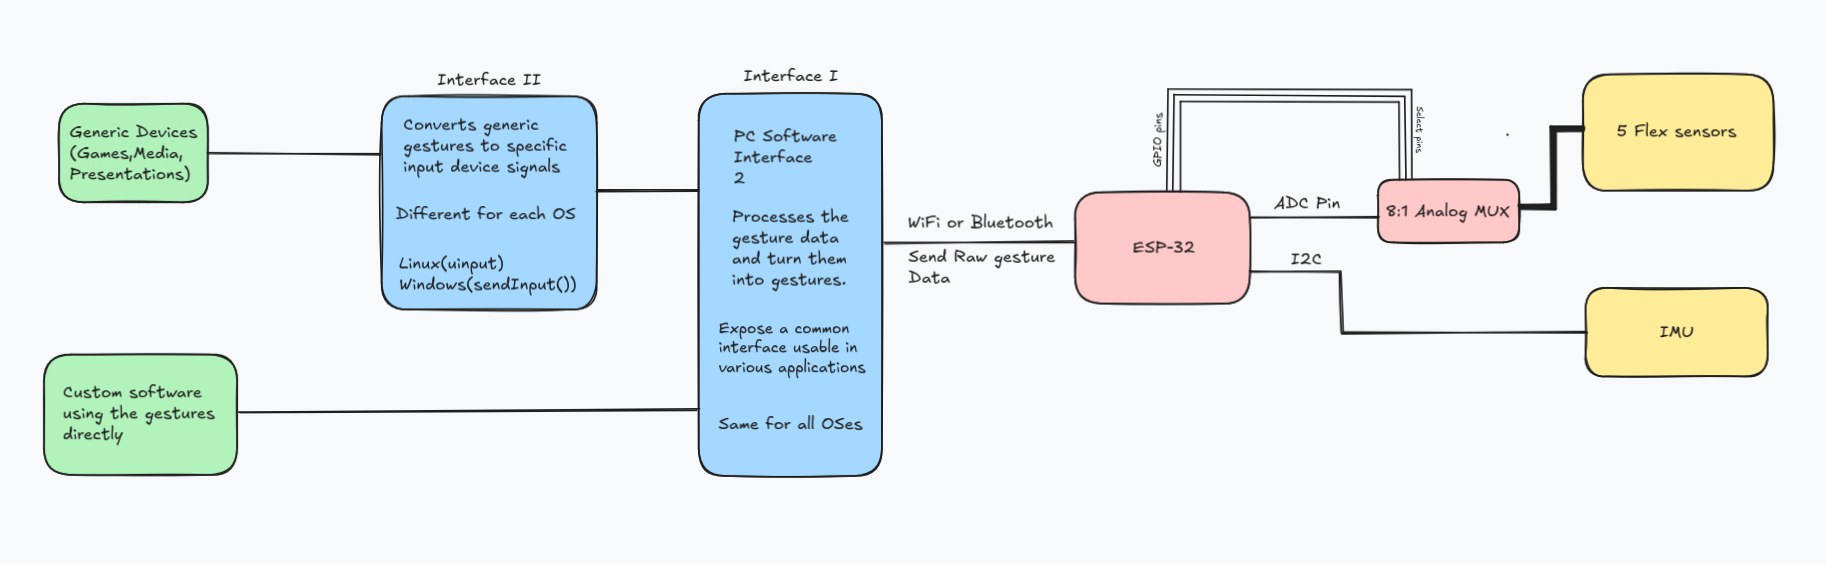
\includegraphics[width=0.95\textwidth]{figures/fig1.png}
\caption{System block diagram: glove sensors → ESP-32 → PC software stack → applications.}
\end{figure}

\subsection{Conditions carried from proposal review}
\begin{tabularx}{\textwidth}{@{}Xll@{}}
\hdrow{Condition / mandatory addition & Status & Where} \\[1pt]
Justify the critical function against $\ge$3 candidates & Done & §2.1 \\
Provide a CDFG with node costs and the critical path & Done & §2.2--2.4 \\
Provide a system FSM with a fault and safe state & Done & §3 \\
State the WCET source and a schedulability proof & Done & §4.1, §4.3 \\
\multicolumn{3}{@{}l@{}}{\footnotesize\color{kicker}All four conditions from the review sheet are closed; the evidence is the corresponding section.}
\end{tabularx}

% ===================== 2 CDFG =====================
\section{Control Data Flow Graph}

\subsection{Choosing the critical function}
\begin{tabularx}{\textwidth}{@{}p{3.4cm}p{2.2cm}p{1.2cm}p{2.2cm}p{1.6cm}X@{}}
\hdrow{Function / ISR & Trigger & Rate & Est.\ exec.\ time & Deadline & Chosen? Why} \\[1pt]
Window inference (features + model.predict) & prediction timer & 4 Hz & $\sim$15 ms & 250 ms & \textbf{Chosen.} Longest execution, most data dependencies, blocks action dispatch. \\
Frame poll (wireless RX) & poll & 30 Hz & $\sim$2--5 ms & 33 ms & No — small, stateless. \\
Frame parse (SimpleBinaryProtocol) & per datagram & 30 Hz & $<$0.5 ms & 33 ms & No — trivial fixed cost. \\
\end{tabularx}

\textbf{Justification:} window inference in
\texttt{backend/app/routers/training.py::predict} has the longest execution
time, consumes the whole buffered window (most data dependencies), and blocks
the action dispatch that follows it.

\subsection{The CDFG}
\begin{figure}[H]
\centering
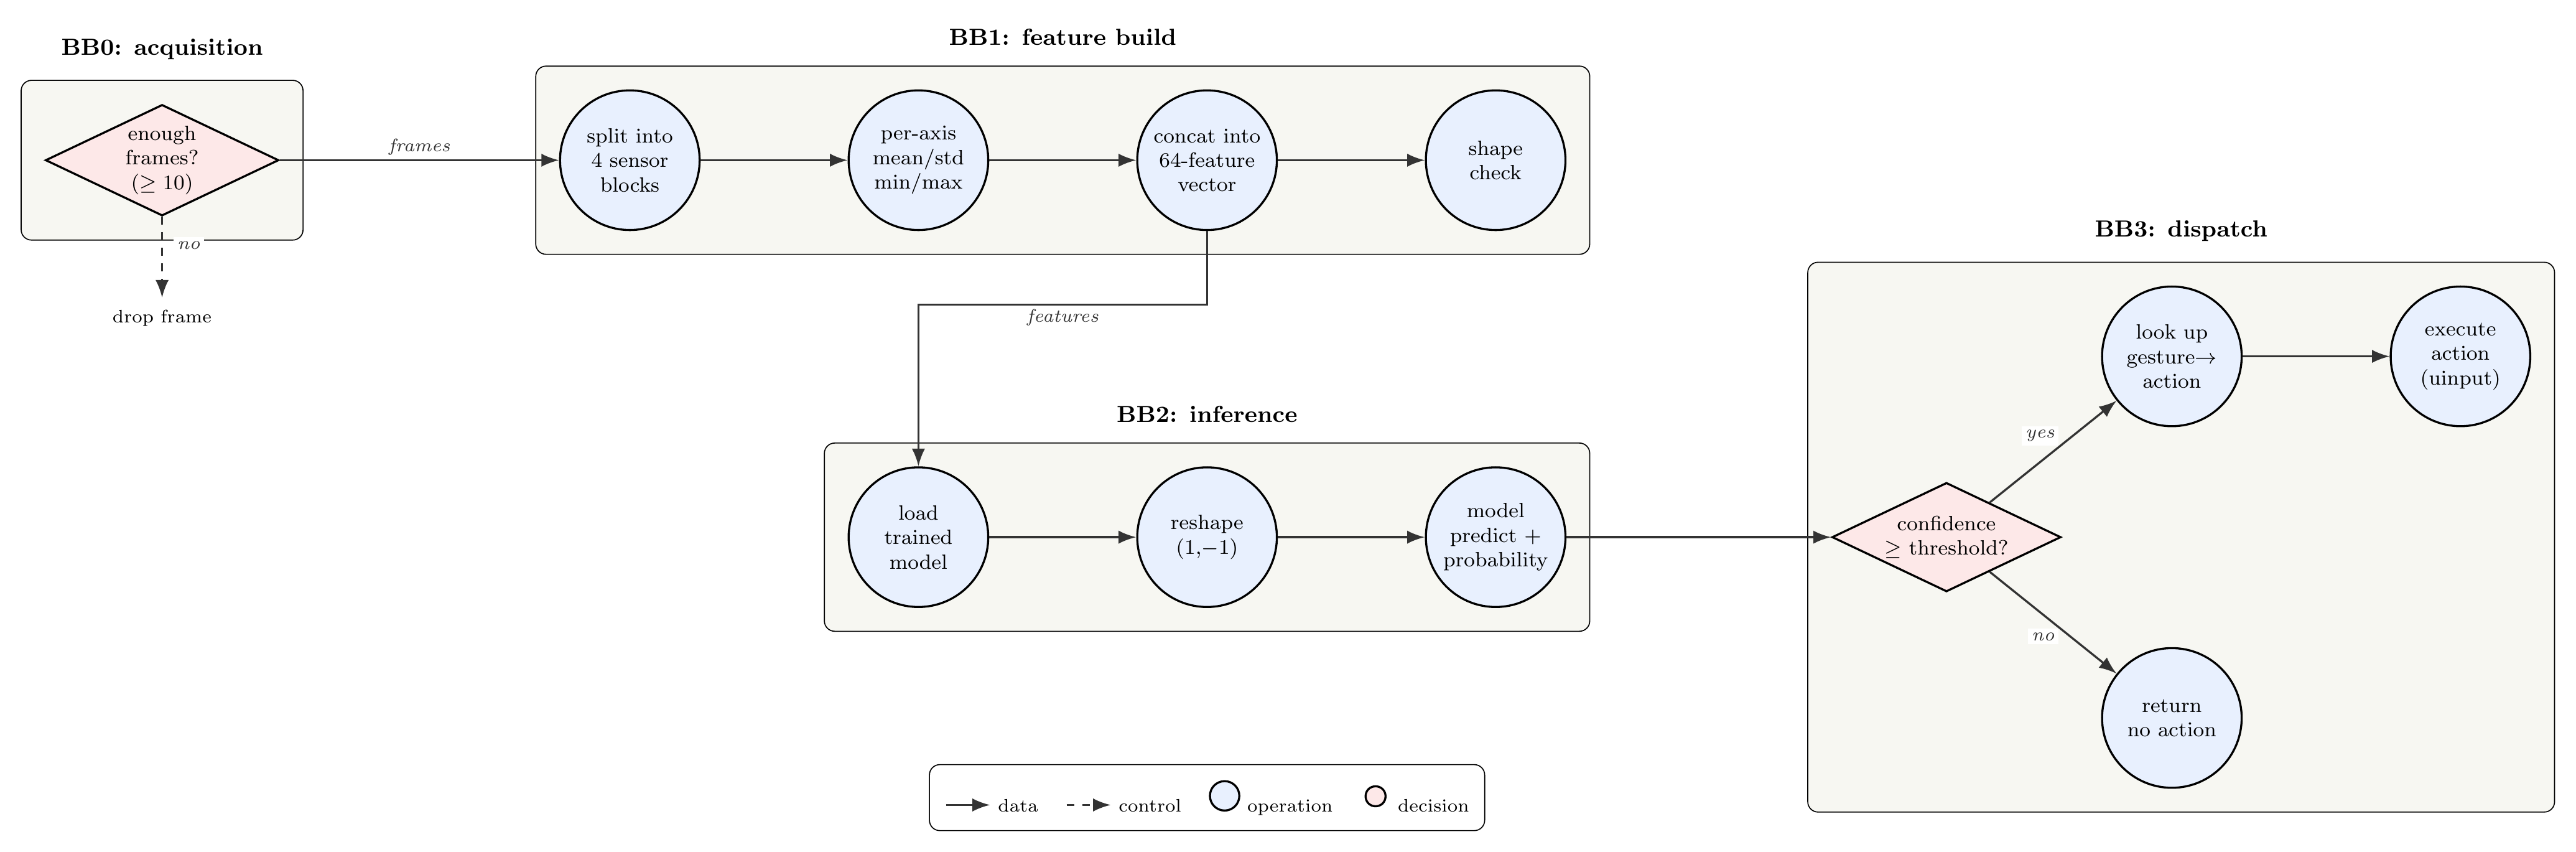
\includegraphics[width=\textwidth]{figures/cdfg-1.png}
\caption{CDFG of \texttt{predict()}. Circles = operations, diamonds = decisions,
solid = data edges, dashed = control edges, grouped into basic blocks BB0--BB3.}
\end{figure}

\subsection{Node table}
\begin{tabularx}{\textwidth}{@{}p{4.0cm}X p{2.4cm}p{1.6cm}@{}}
\hdrow{Operation & Inputs / output & Est.\ cost ($\mu$s) & Function} \\[1pt]
Check window $\ge$10 frames & frame buffer / drop & 200 & \texttt{predict} \\
Split into 4 sensor blocks & frames / blocks & 400 & \texttt{extract\_features} \\
Per-axis mean/std/min/max & block / 4 stats/axis & 2500 & \texttt{extract\_features} \\
Concat into 64 features & stats / vector & 300 & \texttt{extract\_features} \\
Shape check vs model & features, model / ok,400 & 100 & \texttt{predict} \\
Load pickled model & path / model & 1500 & \texttt{predict} \\
Reshape (1,$-$1) & features / 2-D array & 50 & \texttt{predict} \\
predict + predict\_proba & features, model / id, conf & 8000 & \texttt{predict} \\
Confidence $\ge$ threshold? & conf, thr / bool & 50 & \texttt{predict\_and\_act} \\
Look up action binding & gesture id / record & 300 & \texttt{predict\_and\_act} \\
Execute action (uinput) & config / input event & 2000 & \texttt{actions/*} \\
\multicolumn{4}{@{}l@{}}{\footnotesize\color{kicker}All costs are estimated (Python-level, dev PC); none measured yet.} \\
\end{tabularx}

\subsection{Critical path}
\begin{tabularx}{\textwidth}{@{}X p{2.4cm}p{2.0cm}p{2.2cm}@{}}
\hdrow{Critical path (node sequence) & Total latency & Deadline & Slack} \\[1pt]
window → split → stats → concat → load → predict → conf → lookup → execute & $\sim$15.3 ms & 250 ms & $\sim$234.7 ms \\
\end{tabularx}

\noindent\textbf{Dependency to break:} the model load (1.5 ms) is on the path
every call because \texttt{predict} re-opens the \texttt{.pkl}. \emph{Yes} — cache
the model at startup in the Final build. Recomputing full-window statistics
(2.5 ms) could be made incremental, but slack is ample, so it is deferred.

% ===================== 3 FSM =====================
\section{System-behaviour FSM}

\subsection{Model type}
\textbf{Mealy.} Outputs depend on state \emph{and} input — a recognised gesture
emits an action only when confidence $\ge$ threshold. A Moore machine cannot
express ``act only if confident''.

\subsection{State diagram}
\begin{figure}[H]
\centering
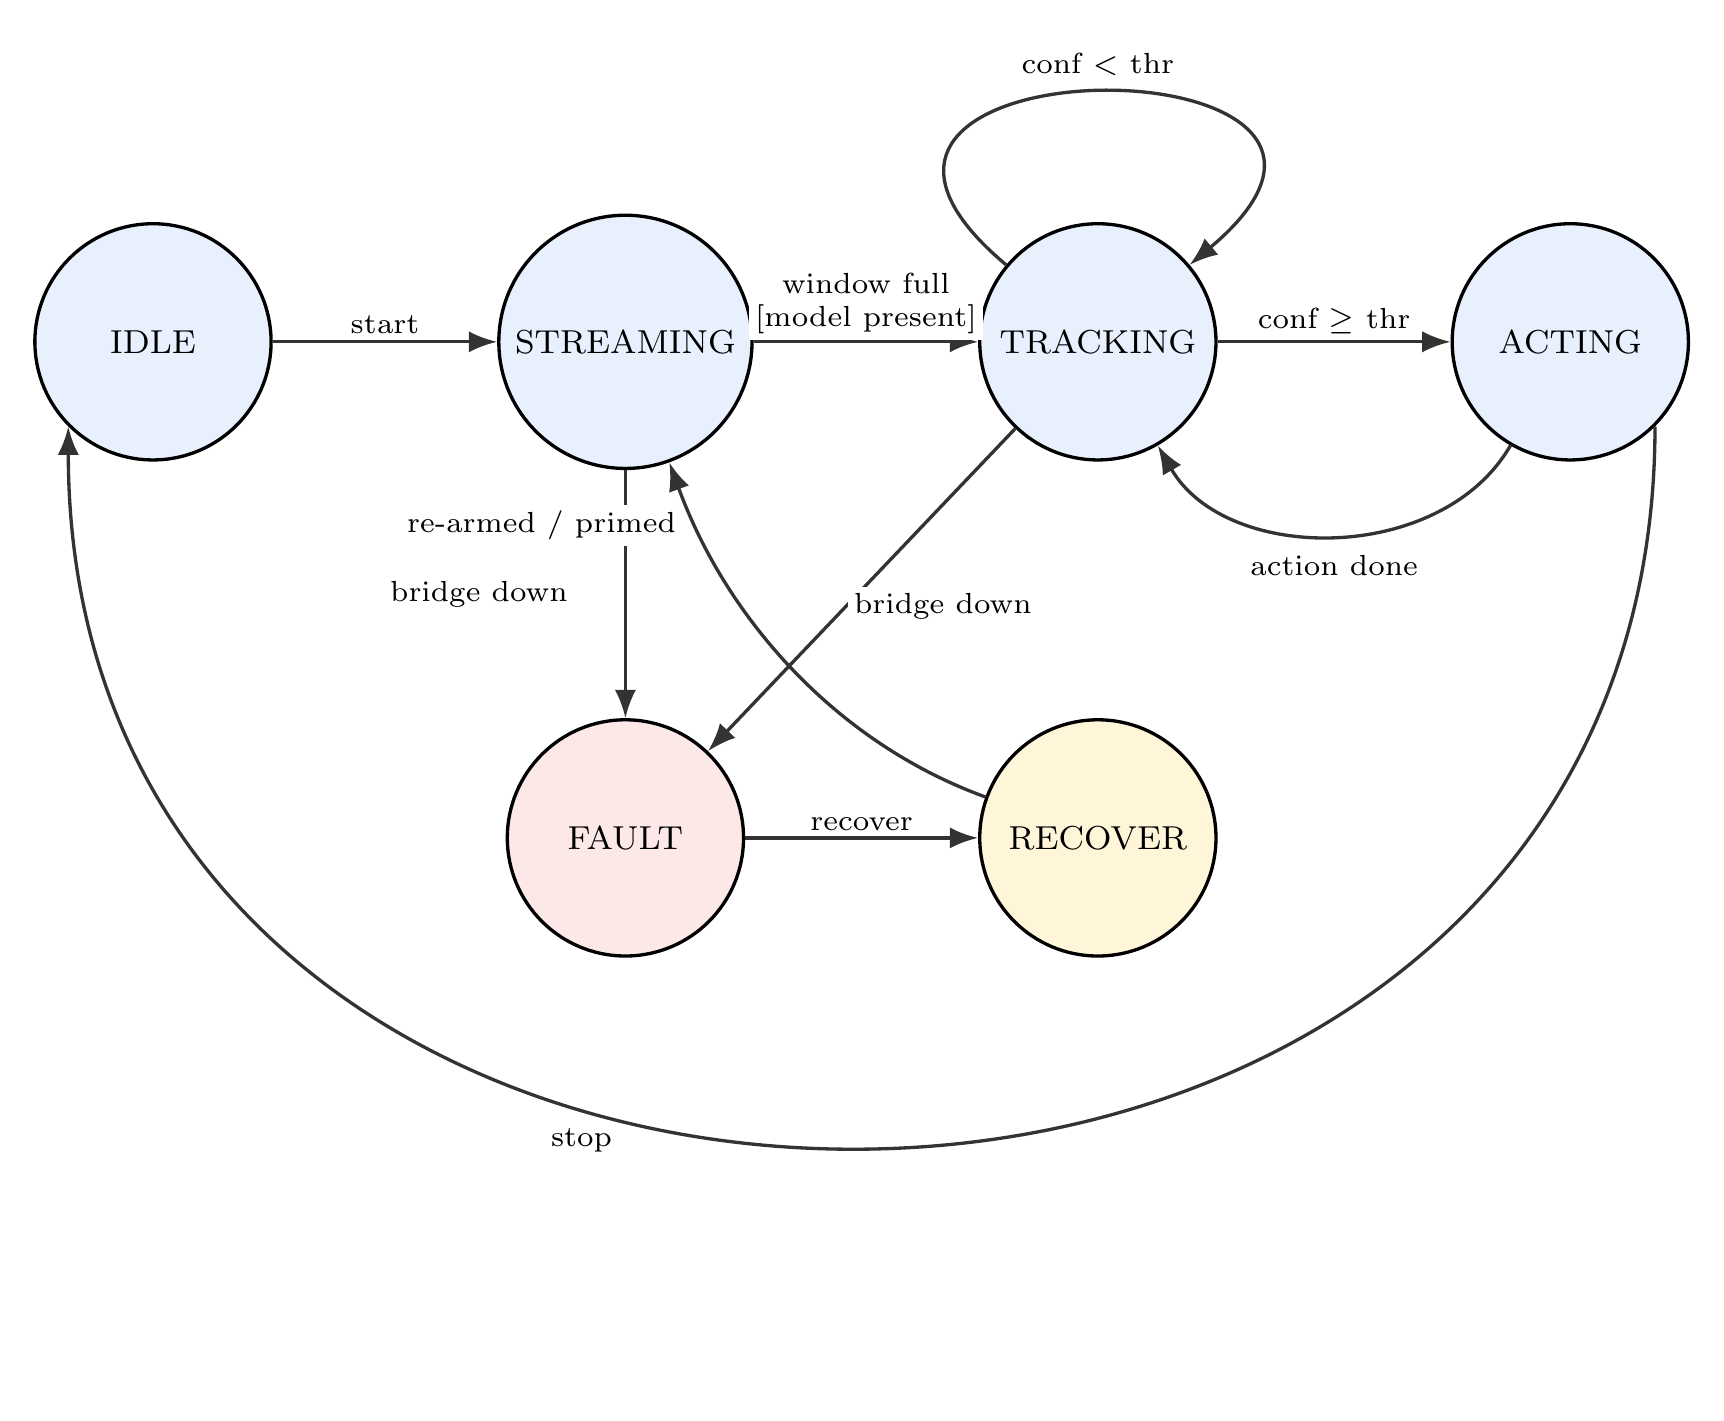
\includegraphics[width=0.62\textwidth]{figures/fsm.png}
\caption{System FSM. Every transition is labelled \texttt{event [guard] / action}.}
\end{figure}

\subsection{State transition table}
\begin{tabularx}{\textwidth}{@{}p{2.2cm}p{2.4cm}p{3.4cm}p{2.2cm}X@{}}
\hdrow{Current state & Event & Guard & Next state & Output / action} \\[1pt]
IDLE & start & sensors available & STREAMING & open transport, buffer \\
IDLE & start & sensors unavailable & FAULT & sensor-unavailable error \\
STREAMING & frame & buffer $<$ window & STREAMING & append frame \\
STREAMING & window full & bridge up, model present & TRACKING & run inference \\
STREAMING & link lost & --- & FAULT & glove-disconnected error \\
TRACKING & tick & confidence $<$ threshold & TRACKING & none (display ``---'') \\
TRACKING & tick & confidence $\ge$ threshold & ACTING & dispatch action \\
ACTING & action done & binding found & TRACKING & inject key/mouse event \\
ACTING & action done & no binding & TRACKING & none (logged) \\
FAULT & recover & link/sensor restored & RECOVER & re-arm, clear buffer \\
FAULT & stop & --- & IDLE & close transport \\
RECOVER & re-armed & buffer primed & STREAMING & resume streaming \\
\end{tabularx}

\subsection{Fault, recovery and safe state}
\textbf{Safe state (FAULT) outputs:} the device emits no keyboard or mouse
events — no key held, no button pressed, no relative motion; every injected event
ends with a release and \texttt{syn()}, so a stuck modifier (e.g.\ held
\texttt{super}) can never lock the desktop. FAULT is reachable from every other
state by the fatal-error / link-loss event. Recovery: \texttt{recover →
RECOVER}, which clears the frame buffer (stale frames must never be inferred
against) and returns to STREAMING only once primed. A watchdog transition
(STREAMING/TRACKING → FAULT on link lost) prevents a dropped wireless link
leaving the system silently half-running.

\subsection{Completeness check}
\begin{tabularx}{\textwidth}{@{}p{2.0cm}XXXX@{}}
\hdrow{State $\downarrow$ / Event $\rightarrow$ & start & frame & window full & tick / bridge-down} \\[1pt]
IDLE & STREAMING & --- & --- & --- \\
STREAMING & --- & STREAMING & TRACKING & FAULT \\
TRACKING & --- & --- & --- & FAULT \\
ACTING & --- & --- & --- & FAULT \\
FAULT & --- & --- & --- & RECOVER \\
RECOVER & --- & --- & STREAMING & FAULT \\
\end{tabularx}

% ===================== 4 TASK SCHEDULE =====================
\section{Task schedule}

\subsection{Task set}
\begin{tabularx}{\textwidth}{@{}p{3.0cm}p{1.9cm}p{1.3cm}p{1.3cm}p{1.3cm}p{1.2cm}p{1.3cm}X@{}}
\hdrow{Task & Trigger & Period T & WCET C & Deadl.\ D & Prio & U & WCET source} \\[1pt]
IMU sampling (MPU-9250) & IMU data-ready / timer & 10 ms & $\sim$0.5 ms & 10 ms & High & 0.050 & datasheet + estimate \\
Flex ADC sampling & ADC timer & 10 ms & $\sim$0.2 ms & 10 ms & High & 0.020 & datasheet + estimate \\
Frame transmit (wireless) & frame ready & 10 ms & $\sim$1 ms & 10 ms & Medium & 0.100 & estimated \\
Frame poll & timer & 33 ms & $\sim$5 ms & 33 ms & High & 0.152 & estimated \\
Inference tick & timer & 250 ms & 15.3 ms & 250 ms & Med & 0.061 & estimated \\
Action dispatch & event & sporadic & $\sim$2 ms & 250 ms & High & 0.008 & estimated \\
Watchdog & timer & 3000 ms & $\sim$1 ms & 3000 ms & Low & 0.0003 & source \\
\end{tabularx}

\noindent\textbf{Total utilisation U $\approx$ 0.23 (23\%).} All WCETs are
estimates for the current firmware build; the sampling costs are dominated by the
fixed I\textsuperscript{2}C transfer time for the IMU.

\subsection{Scheduling approach}
\textbf{Task level: Rate-Monotonic (RMS). Operation level: ASAP list
scheduling.} The task set is small, fixed-rate and preemption-cheap, so RMS
static priorities are simple and provable. EDF would allow higher utilisation
but needs dynamic sorting and response-time checks; at U $\approx$ 0.23 it buys
nothing. A cyclic executive adds jitter without benefit. ASAP gives the shortest
schedule for a mostly-serial CDFG chain.

\subsection{Schedulability analysis}
RMS utilisation bound $U \le n(2^{1/n}-1)$, $n=3$ (poll, inference, watchdog):
\[
\text{bound} = 3(2^{1/3}-1) = 0.7798,\qquad
U = \tfrac{5}{33}+\tfrac{15.3}{250}+\tfrac{1}{3000} = 0.2130 \le 0.7798.
\]
The task set is \textbf{schedulable}. Worst-case response for the inference
task: $R \approx 15.3 + 5$ (one poll interference) $= 20.3$ ms $\ll$ 250 ms
(slack $\approx$ 229.7 ms), so no response-time analysis is required. ASAP
control-step chain: window → split → stats → concat → load → predict → conf →
lookup → execute; all zero mobility except the model load, removable by caching.

\subsection{Timeline}
\begin{figure}[H]
\centering
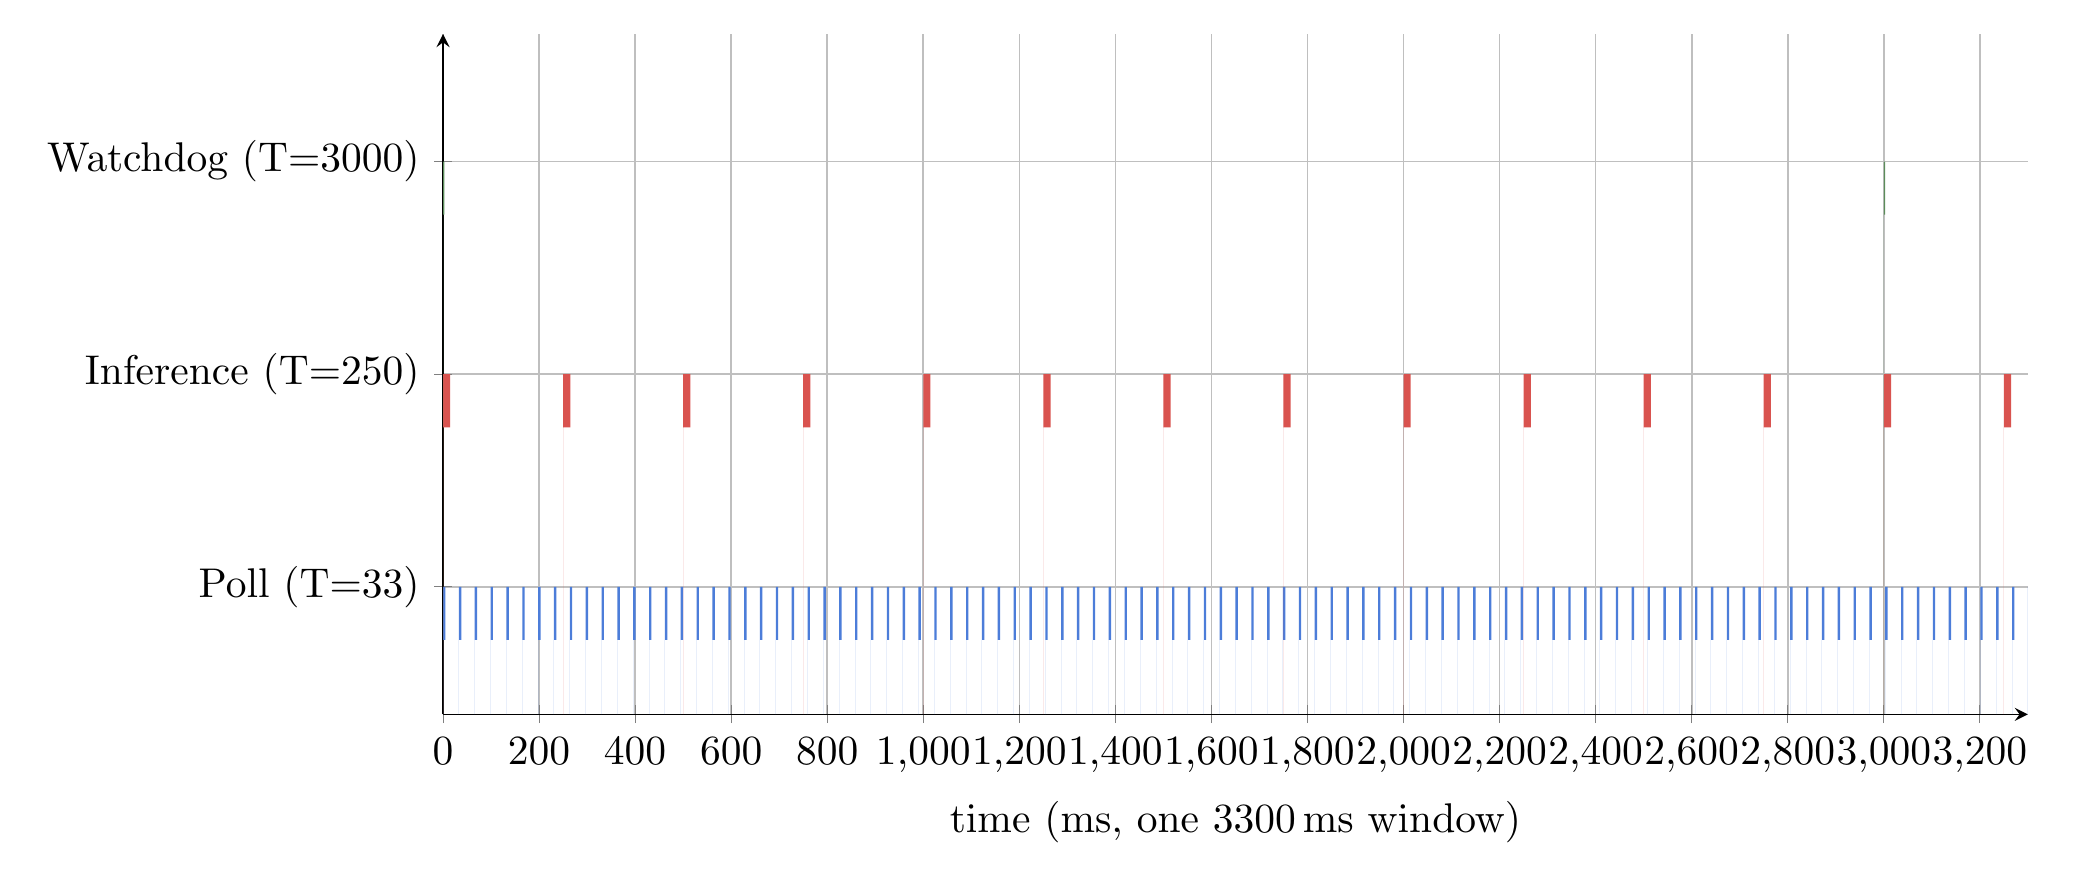
\includegraphics[width=0.92\textwidth]{figures/sched-1.png}
\caption{Schedule over one hyperperiod (task level): poll @33 ms, inference
@250 ms, watchdog @3000 ms; each inference bar sits well inside its frame.}
\end{figure}

\subsection{Shared resources and interrupts}
\begin{tabularx}{\textwidth}{@{}p{3.4cm}p{4.0cm}p{3.4cm}X@{}}
\hdrow{Shared resource & Used by & Protection & Worst-case blocking} \\[1pt]
SQLite \texttt{glove.db} & record / train / predict & session per request & one transaction; no ISR shares it \\
Frame buffer & poll (write), inference (read) & single-threaded & none observed \\
Model \texttt{.pkl} & inference, retrain & load-per-request & $\sim$1.5 ms (removed by caching) \\
uinput device & action dispatch & one UInput/action; \texttt{syn()} & serialised by OS input layer \\
Wireless RX ring buffer & firmware TX / PC RX task & single-producer ring & one buffer copy \\
\end{tabularx}

% ===================== 5 TRACEABILITY =====================
\section{Planned traceability}
\begin{tabularx}{\textwidth}{@{}X p{4.6cm}p{3.6cm}p{1.0cm}@{}}
\hdrow{Model element & Planned file & Planned function & Owner} \\[1pt]
Window guard & \texttt{PredictUI.js} & runPrediction & DJ \\
Feature build & \texttt{training.py} & extract\_features & DJ \\
Inference & \texttt{training.py} & predict & DJ \\
Dispatch & \texttt{training.py} & predict\_and\_act & DJ \\
Input injection & \texttt{input/keyboard.py, mouse.py} & tap / click & DJ \\
FSM states & \texttt{stateMachine.js} (new) & --- & SA \\
Frame poll task & \texttt{backend/app/bridge.py} & get\_latest\_grouped & SA \\
Inference tick task & \texttt{PredictUI.js} & setInterval(…,250) & DJ \\
Watchdog task & \texttt{frontend/src/components/RecordingUI.js} & checkBridge & SA \\
IMU sampling task & ESP-32 firmware & \texttt{imu\_read()} & DJ \\
Flex ADC task & ESP-32 firmware & \texttt{flex\_read()} & DJ \\
\end{tabularx}

% ===================== 6 PLAN =====================
\section{Plan to Final}
\begin{tabularx}{\textwidth}{@{}X p{1.4cm}p{2.0cm}X@{}}
\hdrow{Remaining work & Owner & Target date & Risk and fallback} \\[1pt]
Cache model in memory & DJ & early Oct & Low; fallback = load per request \\
Extract FSM module & SA & early Oct & Medium; fallback = FSM stays implicit \\
Integrate ESP-32 + MPU-9250 + flex on the glove & DJ & mid Oct & High (hardware); fallback = IMU-only \\
Measure WCETs & DJ & mid Oct & Medium; fallback = keep estimates \\
Fault-state unit tests & SA & late Oct & Low \\
\end{tabularx}

% ===================== 7 CONTRIBUTION =====================
\section{Individual contribution}
\begin{tabularx}{\textwidth}{@{}p{3.6cm}X p{4.2cm}p{1.4cm}@{}}
\hdrow{Member & Model / section produced & Module for Final & Share \%} \\[1pt]
Dayakrishn Joshi & System recap, CDFG, task set & ESP-32 firmware + ADC acquisition & 50 \\
Syed Mohammad Ayaan & System FSM, schedulability, traceability, plan & ESP-32 WiFi/UDP link + PC recognition pipeline & 50 \\
\end{tabularx}

% ===================== REFERENCES =====================
\section*{References}
\small
\begin{enumerate}[leftmargin=1.4em,itemsep=2pt]
\item Espressif Systems, \emph{ESP32 Series Datasheet}, 2024.
\item InvenSense, \emph{MPU-9250 Nine-Axis (Gyro + Accelerometer + Compass) MEMS MotionTracking Device Datasheet}, 2016.
\item InvenSense, \emph{MPU-9250 Register Map and Descriptions}, rev.~1.4, 2016.
\item C.~L.~Liu and J.~W.~Layland, ``Scheduling Algorithms for Multiprogramming in a Hard-Real-Time Environment,'' \emph{J. ACM}, 20(1):46--61, 1973.
\end{enumerate}

\end{document}
